\begin{pastexam}[label={px:ust-113-ee-ds-19}]{臺聯大電機類 113 學年度 問答題第 3 題}
（問答；10 分）

Given the following codes, please answer the three questions
\begin{enumerate}[label=(\Alph*)]
\item What is the algorithm that the codes are implemented for? (3 points)
\item What does the graph look like? (3 points)
\item What is the output of the codes? (4 points)
\end{enumerate}
\begin{minted}[fontsize=\small, style=perldoc, breaklines]{java}
import java.util.*;
class process {
    private static final int V = 5;
    int minKey(int key[], Boolean mstSet[]) {
        int min = Integer.MAX_VALUE, min_index = -1;
        for (int v = 0; v < V; v++)
            if (!mstSet[v] && key[v] < min) {
                min = key[v];
                min_index = v;
            }
        return min_index;
    }
    void print(int parent[], int graph[][]) {
        System.out.println("Edge \tWeight");
        for (int i = 1; i < V; i++)
            System.out.println(parent[i] + " - " + i + "\t" + graph[i][parent[i]]);
    }
    void dowork(int graph[][]) {
        int parent[] = new int[V];
        int key[] = new int[V];
        Boolean mstSet[] = new Boolean[V];
        for (int i = 0; i < V; i++) {
            key[i] = Integer.MAX_VALUE;
            mstSet[i] = false;
        }
        key[0] = 0;
        parent[0] = -1;
        for (int count = 0; count < V - 1; count++) {
            int u = minKey(key, mstSet);
            mstSet[u] = true;
            for (int v = 0; v < V; v++)
                if (graph[u][v] != 0 && !mstSet[v] && graph[u][v] < key[v]){
                    parent[v] = u;
                    key[v] = graph[u][v];
                }
        }
        print(parent, graph);
    }
    public static void main(String[] args) {
        process p = new process();
        int graph[][] = new int[][] {
                { 0, 2, 0, 6, 0 },
                { 2, 0, 3, 8, 5 },
                { 0, 3, 0, 0, 7 },
                { 6, 8, 0, 0, 9 },
                { 0, 5, 7, 9, 0 } };
        p.dowork(graph);
    }
}
\end{minted}
\end{pastexam}

\begin{pastsoln}
\textbf{(A)} Prim 演算法，求最小生成樹（資結書第~24.3~節，用陣列找最小 $\mathit{key}$ 的版本，資結書
虛擬碼~24.5）。 $\mathit{key}[v]$ 是「把 $v$ 接到目前的樹上最便宜要多少」，$\mathit{parent}[v]$ 是那條邊的
另一端，$\mathit{mstSet}[v]$ 表示 $v$ 已經在樹上。 每一輪用 \texttt{minKey} 挑 $\mathit{key}$ 最小、還不在樹上
的頂點加入，再用它的邊更新其他頂點的 $\mathit{key}$。

\textbf{(B)} \texttt{graph} 是 $5$ 個頂點的無向加權圖的鄰接矩陣（對稱，$0$ 表示沒有邊）。 共 $7$ 條邊：
$(0,1)\,2$、$(0,3)\,6$、$(1,2)\,3$、$(1,3)\,8$、$(1,4)\,5$、$(2,4)\,7$、$(3,4)\,9$。 粗線是 (C) 求出的最小生成樹。

\begin{center}
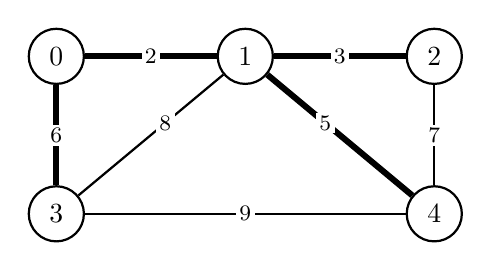
\begin{tikzpicture}[
    v/.style={circle, draw, thick, minimum size=7mm, inner sep=0pt},
    w/.style={fill=white, inner sep=1.2pt, font=\footnotesize},
    e/.style={thick}, t/.style={line width=2.2pt}]
\node[v] (0) at (0,2) {0};
\node[v] (1) at (2.4,2) {1};
\node[v] (2) at (4.8,2) {2};
\node[v] (3) at (0,0) {3};
\node[v] (4) at (4.8,0) {4};
\draw[t] (0) -- node[w] {2} (1);
\draw[t] (0) -- node[w] {6} (3);
\draw[t] (1) -- node[w] {3} (2);
\draw[e] (1) -- node[w, pos=0.4] {8} (3);
\draw[t] (1) -- node[w, pos=0.4] {5} (4);
\draw[e] (2) -- node[w] {7} (4);
\draw[e] (3) -- node[w] {9} (4);
\end{tikzpicture}
\end{center}

\textbf{(C)} 追蹤 \texttt{dowork}（$\infty$ 表示 \texttt{Integer.MAX\_VALUE}，「$-$」表示還沒設定）。 每一列是
那一輪挑出 $u$、更新完之後的狀態：
\begin{center}
\small
\begin{tabular}{cc ccccc ccccc}
\toprule
& & \multicolumn{5}{c}{$\mathit{key}[0..4]$} & \multicolumn{5}{c}{$\mathit{parent}[0..4]$} \\
\cmidrule(lr){3-7}\cmidrule(lr){8-12}
\texttt{count} & $u$ & 0 & 1 & 2 & 3 & 4 & 0 & 1 & 2 & 3 & 4 \\
\midrule
開始 & & 0 & $\infty$ & $\infty$ & $\infty$ & $\infty$ & $-1$ & $-$ & $-$ & $-$ & $-$ \\
0 & 0 & 0 & 2 & $\infty$ & 6 & $\infty$ & $-1$ & 0 & $-$ & 0 & $-$ \\
1 & 1 & 0 & 2 & 3 & 6 & 5 & $-1$ & 0 & 1 & 0 & 1 \\
2 & 2 & 0 & 2 & 3 & 6 & 5 & $-1$ & 0 & 1 & 0 & 1 \\
3 & 4 & 0 & 2 & 3 & 6 & 5 & $-1$ & 0 & 1 & 0 & 1 \\
\bottomrule
\end{tabular}
\end{center}
說明：$u = 1$ 時，$(1,3)$ 的 $8$ 不小於 $\mathit{key}[3] = 6$，不更新；$u = 2$ 時 $(2,4)$ 的 $7$ 不小於
$5$；$u = 4$ 時 $(4,3)$ 的 $9$ 不小於 $6$。 迴圈只跑 $V - 1 = 4$ 輪，最後一個頂點 $3$ 沒有被標進
$\mathit{mstSet}$，但它的 $\mathit{parent}[3] = 0$ 已經不會再變，所以不影響結果。

\texttt{print} 印出（\texttt{\textbackslash t} 是 tab 字元，下面用空白對齊表示）：
\begin{minted}[fontsize=\small]{text}
Edge    Weight
0 - 1   2
1 - 2   3
0 - 3   6
1 - 4   5
\end{minted}
最小生成樹的總權重是 $2 + 3 + 6 + 5 = 16$。 \texttt{graph[i][parent[i]]} 和 \texttt{graph[parent[i]][i]}
一樣（矩陣對稱），印出的就是那條樹邊的權重。
\end{pastsoln}
